\chapter{A Proposal for a Future Predictive Model -- A Bayesian Hierarchical Approach}
  \label{ch:bayes}
% alt:A Bayesian Hierarchical Predictive Soundscape Model and a Proposed Soundscape Index
% alt: Probabilistic soundscape models including personal, contextual, environmental, and acoustic information

\section{Introduction}
\subsection{The problem with the pleasant-annoying paradigm}

As made clear by their name, noise annoyance studies have focussed on the relationship between noise (or acoustic) features and the perceived annoyance, to varying degrees of success. Within the soundscape circumplex framework, annoyance is the negative side of the pleasantness dimension, forming the \nth{1} primary component of soundscape perception. This means that, along with pleasantness, annoyance is that perceptual attribute which is most readily perceived and plays the largest part in differentiating between the perception of different soundscapes. This fact therefore makes this pleasantness dimension the prime target for addressing noise issues. 

However, \citet{Mitchell2021Investigating} (i.e. \cref{ch:lockdown}) and \citet{Aumond2022} have both recently demonstrated a fundamental difference in the statistical relationships connecting context and acoustic features with the perceived pleasantness and eventfulness of urban soundscapes. %TODO: Continue this discussion about including eventfulness. Can draw from that review I wrote

\section{Starting point} 
\draft{The lockdown model, as the most developed model so far.}

\section{Incorporating personal factors into a predictive soundscape model}
Although, as \citet{Droumeva2021sound} points out, each individual brings their own cultural and subjective aspects of listening to the stage of urban sound, when attempting to characterise the soundscape of a space, it is not a particular individual's aspects we should be concerned with. That individual forms a part of the collective perception of the space. Their cultural and subjective (i.e. personal) aspects mitigate their perception, but this perception then forms only a single component of the collective perception. How then should we consider these personal factors? Surely there is no suggestion to disregard their influence and importance within the soundscape approach? In my view, there are two approaches:

\begin{enumerate}
  \item Incorporate these personal factors as demographic statistics of a location; or
  \item An agent-based approach where each individual likely to use the space is simulated and modelled with their personal factors to then be included in the collective perception.
\end{enumerate}

Let's look at how these two approaches would be implemented in a multilevel acoustics-based predictive model, such as those presented in \crefrange{ch:mlmann}{ch:lockdown}.

%TODO: Expand
\subsection{Approach 1}
In the first, the demographic breakdown of the space under investigation is estimated, either through a census or by the designers' desired use case. This demographic breakdown can then be compared to the results presented above \citep{Erfanian2021Psychological} to derive weighting factors which adjust the predicted soundscape assessment. For instance, the results suggest that retired persons perceive the soundscape as \draft{XX\% or amount [need to check with results]} less pleasant than others. If the particular space under investigation has a large proportion of retired persons, say 65\% we could then apply an adjustment to the initial personal-factors-agnostic prediction to reflect this tendency. In this example, an initial location-level \gls{isopl} prediction of 0.36, with a 65\% retired population would be corrected by \draft{-XX [0.65 x result]} for a final demographics-corrected \gls{isopl} prediction of \draft{XX}.

\subsection{Approach 2}

\subsection{Benefits and downsides of each approach}

\section{Incorporating sound source information}

\section{Probabilistic predictions - A Bayesian Approach?}

\subsection{Defining a distribution}

\subsubsection{Truncated normal distribution}

Given that the \gls{isopl} and \gls{isoev} values have a hard boundary at $[-1, +1]$, it is not in fact correct to consider the distribution of responses within the circumplex as a normal distribution. A normal distribution is defined as extending out to $(-\infty, \infty)$ with an area of 1 under the probability density. If the potential space of the responses is bounded, the assumption of them forming a normal distribution is violated, as part of the probability density function is unreachable, meaning the area under the probability density will not sum to 1.

If we assume the general shape of the responses to be normal, then they would instead form a truncated normal distribution \cit{\url{https://people.sc.fsu.edu/~jburkardt/presentations/truncated_normal.pdf}, \url{https://www.tandfonline.com/doi/abs/10.1080/00031305.1999.10474490}}. Briefly, a truncated normal distribution is estimated by first calculating the probability density function of the standard normal distribution. Then, the density function is truncated at the set boundary ($[a, \infty)$ or $(-\infty, b]$) or boundaries ($[a, b]$) and the portion of the density function which is truncated is redistributed within the boundary.

This redistribution means that the various parameters of a truncated distribution will be somewhat different than for a normal distribution, in particular the calculation of variance. This impacts the soundscape distribution plots demonstrated in \cref{ch:circumplex} as the kernel density estimation performed by the underlying plotting library (\texttt{seaborn}) assumes a normal distribution with no boundary. It is possible that making use of a truncated normal distribution would change the shape of the distributions produced by \texttt{soundscapy}. Although at this point there does not seem to be a simple method of adapting the \texttt{soundscapy} code to make use of a truncated distribution, I chose to briefly test out how much of a change the truncated distribution is likely to make to the shape of the \texttt{soundscapy} plots through functions available in \texttt{R}. 

\begin{figure}
  \centering
  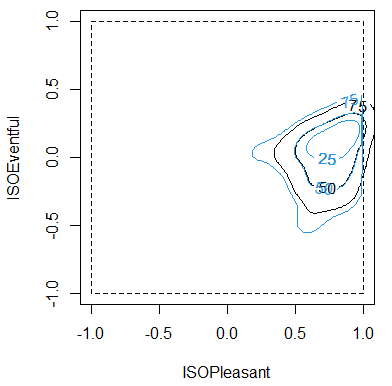
\includegraphics{Figures/Trunc-Normal-demo.png}
  \caption{Comparing a probability distribution in the soundscape circumplex (using Regents Park Japan as the worst case example) using a normal kernel density estimation method (black line) and a truncated KDE (blue line). \label{fig:truncatekde}}
\end{figure}

From \cref{fig:truncatekde}, it appears that there would be some difference in the shape of the soundscape distribution when using a truncated distribution. However, I would note that Regents Park Japan was chosen as the worst case location in the whole \gls{isd} as the samples lie closest to the boundary and the density function estimated in \texttt{soundscapy} has the most area which lies outside the boundary. Most locations do not show any overlap with the boundary and would not be noticeably affected by the truncation. In addition, switching to the truncated normal distribution only affects those iso-density levels which overlap with the boundary. Therefore, the recommended simplified density curve given in \cref{ch:circumplex} of 50\% is effectively unchanged since it is very unlikely the \nth{50} percentile curve would exceed the boundaries. For the time-being, therefore it appears that there is not a detriment to using a standard normal distribution as opposed to a truncated normal distribution, for the visualisations created by \texttt{soundscapy}.

However, as I move towards a probabilistic prediction framework, and even in the frequentist predictive models used throughout this thesis, it seems possible that the distinctions between these underlying distributions will become more important. 


\section{Discussion}

\section{Conclusion}

